\section{Introduction}
As AI progresses from olympiad problems to research proofs, what changes in our expectations about an open conjecture, an unsolved algorithmic problem, or a cancer treatment? Predicting what comes next requires knowing which target requirements a system can meet and what validation remains. This question arises within mathematics as well as between mathematics and biomedicine.

Consider a procedure that selects a compound and tests it in a specified cell assay. A mathematical breakthrough alone does not tell us how reliably this procedure will find a confirmed hit. Even if that reliability can be predicted, two further questions remain: when will a suitable procedure become available, and when will selection and validation finish? The procedure available first need not be most likely to finish by a deadline (\S\ref{sec:domains}). This comparison is hypothetical; patient benefit requires a different target.

Our position is that a computational theory of scientific discovery should connect capability growth to the changing set of achievable targets and to their eventual completion. We first need a target response: how measured capability relates to the chance of validated success. Combining that response with a scenario for future capabilities and resources gives an availability date. Deployment and validation then determine completion. A breakthrough can inform the target response without settling these later stages. Researchers need target measurements before extrapolation and validation schedules before choosing a procedure. An unknown date does not mean the target is unsolvable.

The assay example supplies exact calculations of measurement and evaluation costs (\S\S\ref{sec:horizons}--\ref{sec:tests}). Two archive studies ask whether task structure or early experimental outcomes improve prediction (\S\S\ref{sec:pathways},\ref{sec:scope}). Their gains and reversals show why added information must be tested on the intended targets. These conditional examples and retrospective tests do not validate a calendar of breakthroughs.

These foundations are established: complexity and learning theory separate computation from information requirements \citep{arorabarak2007,shalev2014,traub1988}; observational scaling predicts downstream performance from capability coordinates \citep{ruan2024}; Sloth connects latent skills to model size and training tokens \citep{polo2025sloth}. ADeLe uses annotated task demands \citep{zhou2026scales}; other predictors use performance histories and validation loss \citep{hu2026neuneu,truong2026irsl}. Capability theories, measurement validity and biomedical acceleration constraints also precede this work \citep{jo2026,wallach2025,hebenstreit2026}. Our synthesis connects these established tools to the choice of scientific procedure and tests where extra target information helps. It introduces no new scaling law: a response model combined with the correct deployment model already implements this position.

\section{Defining the target and its conditions}
\label{sec:complexity}
\subsection{Define the scientific event and its resources}
A target $Q$ specifies the problem or instance population and the validated outcome to be produced. Its success probability can refer to two settings. For a declared distribution of problem instances, success is averaged over those instances. For one fixed problem, the probability instead concerns randomness in the procedure and its observations.

For the assay, fix a cell line, viability threshold and repeat-assay confirmation rule before selecting compounds. The target is one compound meeting that rule; an attempt includes selection and validation. A correct candidate somewhere in a generated set does not establish that the procedure can select and validate it \citep{dorner2026roc}. A causal mechanism or patient benefit would be a different target. Likewise, proving a supplied statement differs from selecting and resolving a significant open conjecture. 

To retain trade-offs between computation, observations and time, we record resource combinations. Let $K$ denote information and observation access, $\Pi$ the permitted procedures, and $\mathbf b$ the resource allowance. A procedure includes its model, tools, orchestration and human assistance. Comparing complete systems permits these to vary; attributing a gain to one component requires controlling the others. For procedure $\pi$, write $p(\pi,Q;\mathbf b,K)$ for its probability of producing a validated result within those limits. At required reliability $q$, define
\begin{equation}
 \mathcal B_Q(q\mid K,\Pi)=\{\mathbf b:\exists\pi\in\Pi,\ p(\pi,Q;\mathbf b,K)\ge q\},\qquad
 \mathcal A_t(q)=\{Q:\mathbf b(t)\in\mathcal B_Q(q\mid K_t,\Pi_t)\}.
 \label{eq:complexityset}
\end{equation}
\label{eq:attainable}
The first set contains sufficient resource combinations; the second gives achievable targets under resources $\mathbf b(t)$, information $K_t$ and procedures $\Pi_t$ available at time $t$. In the assay example, computation, allowed assays and elapsed validation time are separate resources. More computation may help select candidates without reducing the duration of their assays. The allowance includes campaign duration, so achievable at time $t$ means a suitable campaign can begin then, not that it has already finished. 

If two procedures need (10 compute units, 10 observations) and (100, 1), their separate minima do not imply that (10, 1) suffices. Existence of a suitable procedure does not mean an evaluator finds it. Inherent computational complexity instead concerns all algorithms in a specified model, often asymptotically. Today's model failure establishes neither an inherent lower bound nor a date for overcoming it.

Required reliability $q$ is a decision requirement, not a complexity estimate. Its choice must reflect the consequences of failure. Mean quality cannot replace success probability, which depends on the validation and selection procedures and their errors.

\subsection{Observation access changes the attainable set}
Some targets require information that the allowed observations cannot supply. Suppose two mechanisms generate identical distributions of observation histories under every permitted adaptive policy, but require opposite binary answers. Every permitted procedure then has the same output distribution in both worlds: choosing one answer with probability $r$ gives accuracies $r$ and $1-r$. Worst-case accuracy is at most $1/2$. This premise constrains every procedure; poor performance by one predictor does not establish it. Distinguishing observations or a justified structural restriction can remove this obstruction; more computation on unchanged evidence cannot. This is an identification argument under explicit observation restrictions, with close connections to causal transport and biological context \citep{bareinboim2016,dibaeinia2026,mccormick2026}.

For example, recover the program $f_a(x)=ax\bmod 2^n$ with uniformly hidden odd $a$. If each rejected candidate only rules out its own coefficient, positive verification with 90\% probability needs $\lceil.9\,2^{n-1}\rceil$ checks. Observing $f_a(1)$ instead reveals $a$. The exponential cost belongs to the restricted interface, not multiplication. Appendix~\ref{app:synthesis} supplies exhaustive checks and verification costs.

\section{From demonstrated capability to target performance}
\label{sec:pathways}
A source score describes a system; it does not describe what a new target demands. We ask whether combining the two improves prediction. A solved problem can reveal relevant ability without transferring its solution. Let $\mathbf z$ be the measured capability profile and $\boldsymbol\kappa_Q(K)$ the target description under access $K$. A shared rule $F_{\boldsymbol\theta}$, with fitted parameters $\boldsymbol\theta$, predicts success from these quantities and the resource allowance. For the assay target, success means one complete selection-and-validation attempt. Our archive tests instead use computational outcomes. The second expression is a restricted logistic example:
\begin{equation}
 \widehat p_Q=F_{\boldsymbol\theta}(\mathbf z,\boldsymbol\kappa_Q(K),\mathbf b),\qquad
 \widehat p_Q=\sigma(\mathbf a_Q^\top\mathbf z-d_Q),\quad \sigma(u)=(1+e^{-u})^{-1}.
 \label{eq:bridge}
\end{equation}
\label{eq:logistic}
The logistic model holds resources, information and protocol fixed. Log-odds are $\log[p/(1-p)]$; a linear relation on this scale becomes a curved probability response. The weights $\mathbf a_Q$ describe how target log-odds vary with measured capabilities; $d_Q$ shifts the response curve. This item-difficulty parameter is not computational complexity. Fix capability units and normalization before comparing coefficients.

For an unseen target, shared functions must determine its coefficients: $\mathbf a_Q=\mathbf a_{\boldsymbol\theta}(\boldsymbol\kappa_Q)$ and $d_Q=d_{\boldsymbol\theta}(\boldsymbol\kappa_Q)$. Fitting separate coefficients after observing each target's outcomes cannot supply that prediction. Even a successful shared fit remains an association: it does not establish that intervening on one capability causes improvement.

\subsection{Testing target descriptions in a common archive}
We use the public ObsScaling archive \citep{ruan2024}. Principal component analysis (PCA) summarizes seven source scores: MMLU, ARC-C, HellaSwag, Winograd, TruthfulQA, GSM8K and XWinograd. PC1 is the first coordinate; PC1--3 uses the first three. Source scores and PC coordinates are standardized on training models only. 

We test a narrower version of the shared-description hypothesis using BIG-Bench Hard (BBH) logical deduction and shuffled-object tracking, each with 3, 5 and 7 objects. The descriptor is log object count, fixed from task definitions. Three-shot chain-of-thought strict-match scores come from the same archive: 73 models in 20 archive-defined groups, each evaluated on six task versions, giving 438 aggregate success rates. These 20 archive groups can share ancestry; their identities are listed in Appendix~\ref{app:empirical}. A cell is a published model--task rate, not one generated answer. We compare PC1 and PC1--3 with count-informed predictors. Adding count shifts predicted log-odds; interactions additionally let capability effects vary with count.

PCA uses each training model once; regressions fit its rates on the available task versions. Prediction inputs are seven measured source scores and, for count-informed fits, target object count. Family labels define exclusions; only the task-family-mean baseline uses task identity as a prediction key. Test rates are withheld. We score predictions by mean squared error against archived success fractions (rate-MSE), not by counting validated discoveries. Table~\ref{tab:descriptor} separates task-family, model-family and size holdouts from joint family exclusion.

\begin{table}[htbp]
\centering\small
\caption{Archived rate-MSE; lower is better. Separate holdouts exclude a task family (438 cells), model family (438), or size 7 (146; training at 3/5). Joint holdout excludes both families (438 cells); Cells weights cells equally, Families weights the 20 model groups equally. Each split uses identical cells across predictors. $\dagger$ marks post-result rivals; the joint test is also post-result. These are retrospective, not contamination-controlled tests.}
\label{tab:descriptor}
\begin{tabular}{lrrrrr}
\toprule
& \multicolumn{3}{c}{Separate holdouts} & \multicolumn{2}{c}{Joint holdout}\\
Predictor & Task & Model & Size & Cells & Families\\
\midrule
Pooled mean & 0.0431 & 0.0427 & 0.0446 & 0.0446 & 0.0532\\
Task-family mean & 0.0431 & 0.0422 & 0.0447 & 0.0446 & 0.0532\\
PC1 & 0.0342 & 0.0320 & 0.0307 & 0.0357 & 0.0432\\
PC1--3 & 0.0355 & 0.0330 & 0.0307 & 0.0379 & 0.0459\\
Count only$^\dagger$ & 0.0395 & 0.0371 & 0.0279 & 0.0410 & 0.0535\\
PC1--3 + count$^\dagger$ & 0.0260 & 0.0234 & 0.0179 & 0.0285 & 0.0356\\
PC1--3 + chance floor$^\dagger$ & 0.0266 & 0.0270 & 0.0217 & 0.0287 & 0.0350\\
PC1--3 + count interactions & 0.0277 & 0.0238 & 0.0195 & 0.0301 & 0.0377\\
\bottomrule
\end{tabular}

\end{table}

In Table~\ref{tab:descriptor}, PC1--3 + count outperforms the interaction model in the three separate holdouts. The chance-floor predictor uses $1/n+(1-1/n)\sigma(\beta_0+\boldsymbol\beta^\top\mathbf z)$ for $n$ objects; it assumes rather than guarantees a floor on LLM accuracy. The task-family mean uses training rates from the same task family, falling back to the pooled mean when that family is withheld. Among these eight, the chance-floor predictor has the lowest task-family cross-entropy (Appendix~\ref{app:empirical}); no new models were evaluated.

\paragraph{One held-out prediction.}
To predict Gemma-7B's seven-object deduction score, we withhold its model group, the deduction family and size 7, then train on 142 tracking rates: 71 non-Gemma models from 19 groups, at 3/5 objects. Gemma-7B's source scores and the target count enter the fitted rule; its deduction outcome does not. PC1--3 predicts $.411$; adding count predicts $.211$. The archived rate is $.376$, giving squared errors $.00120$ and $.02720$. This example shows how one prediction is scored; it does not represent the average effect. Figure~\ref{fig:joint_main} summarizes all such exclusions, including the pooled benefit and deduction reversal.

\begin{figure}[htbp]\centering
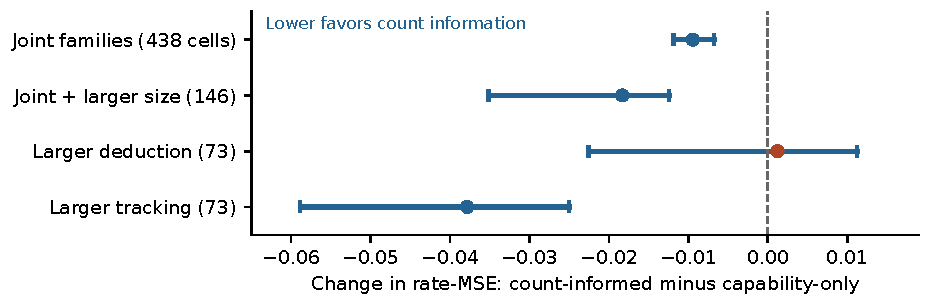
\includegraphics[width=\linewidth]{figures/joint_effects_main.pdf}
\caption{Does object count improve prediction when both model and task families are withheld? Dots show the rate-MSE of PC1--3 + count minus that of PC1--3; negative favors adding count. Bars are 95\% percentile ranges from 500 model-family refits, not uncertainty over new task families. The last two rows partition the 146-cell size-extrapolation test. Deduction worsens at the observed point estimate and its interval spans zero.}
\label{fig:joint_main}
\end{figure}

PC/count fits minimize the sum of squared residuals on logits of target rates clipped to $[.005,.995]$, plus the sum of squared non-intercept coefficients (ridge penalty 1). Log count is standardized on training cells. Coefficients are shared across task versions; the intercept is unpenalized. The penalty is fixed, not tuned on held-out outcomes.

At seven objects, adding count changes tracking rate-MSE from $.06159$ to $.02375$, but deduction from $.01680$ to $.01802$ (73 cells each; Figure~\ref{fig:joint_main}). This establishes a target-description association, not a computational-complexity mechanism: count also changes the answer space. A forecast for a new target needs a relevant transfer test, not just a better pooled score.

The preferred predictor also depends on whom the average represents. In Table~\ref{tab:descriptor}, additive count narrowly beats the chance floor when cells receive equal weight ($.02845$ vs. $.02873$), but loses when each model family gets weight $1/20$ ($.03558$ vs. $.03503$). Rankings therefore depend on the error measure, weighting and holdout. The pooled count gain survives alternative fits (probit, direct rate prediction, clipping thresholds and a quadratic capability-only rival), but adding count to the chance-floor predictor is not uniformly better.

Figure~\ref{fig:joint_main}'s ranges concern model-family sensitivity with two fixed task families and no item-level outcomes (Appendix~\ref{app:robustness}). A date forecast additionally needs a capability-growth trajectory.

\section{From target performance to a conditional date}
\label{sec:horizons}
\subsection{The missing relation and how to measure it}
A response curve gives success at a capability level; a date asks when that procedure becomes available. For the assay, require a complete single-candidate procedure to pass with probability at least $q$, rather than reaching $q$ through many attempts. For fixed reliability and a development scenario, define the earliest availability time as
\begin{equation}
 \tau_Q(q)=\inf\{t\ge0:Q\in\mathcal A_t(q)\}.
 \label{eq:horizon}
\end{equation}
If no permitted procedure ever meets the target, $\tau_Q=\infty$. This date concerns availability; a campaign need not start then. Each scenario below permits one procedure; admitting alternatives cannot delay the earliest availability date. A probabilistic forecast would also need uncertainty about capability growth, target response, resources and access.

The following values are hypothetical. Here $p_Q$ is single-attempt success and $q$ its required threshold; $\lambda$ measures log-odds change per capability unit, $v$ capability units per year, and $\tau_Q$ years to availability. Section~\ref{sec:tests} instead uses $\rho$ for a multi-attempt campaign hit probability. With initial log-odds $\eta_0$ and a fixed linear relation,
\begin{equation}
 \operatorname{logit}p_Q(t)=\eta_0+\lambda vt,\qquad
 \tau_Q(q)=\frac{\operatorname{logit}q-\eta_0}{\lambda v}.
 \label{eq:crossing}
\end{equation}
The finite crossing formula assumes $v,\lambda>0$ and initial success below $q$. With $\eta_0=-3$, $v=1$ and $q=.8$, procedures A and B with slopes (couplings) $\lambda=1$ and $.5$ become available after 4.39 and 8.77 scenario-years; a zero-coupling procedure never does. All three agree on the source trajectory and current target success $.0474$. At one additional source unit, A and B instead predict $.1192$ and $.0759$: a matched target measurement can begin to distinguish them, subject to sampling error. Thus source progress and current target performance do not identify the horizon when coupling is unrestricted. Appendix Figure~\ref{fig:horizons} displays these constructed curves. 



\paragraph{A constructive measurement procedure.}
Measuring the target at two capability levels supplies information missing from a single current success rate. Assume log-odds vary linearly with capability. Use the same target protocol at levels separated by $\Delta>0$, with $N$ independent success/failure trials at each level. Form individual 97.5\% Clopper--Pearson intervals $[L_0,U_0]$ and $[L_1,U_1]$ by allocating .0125 to each of four tails, giving at least 95\% simultaneous coverage \citep{clopper1934}.

Subscripts 0 and 1 denote lower and higher capability. To bound improvement conservatively, pair the lower success bound at higher capability ($L_1$) with the upper bound at lower capability ($U_0$); reverse the endpoints for the largest change. On the log-odds scale, dividing by the capability separation gives
\begin{equation}
 \lambda\in\left[\frac{\operatorname{logit}L_1-\operatorname{logit}U_0}{\Delta},
 \frac{\operatorname{logit}U_1-\operatorname{logit}L_0}{\Delta}\right].
 \label{eq:lambda_interval}
\end{equation}
Across repeated samples at these fixed levels, at least 95\% of intervals cover the slope if the binomial and affine-logit premises hold; this is not 95\% coverage of a future discovery date. Zero successes or all successes at a level can leave an interval endpoint infinite. Cross-level independence is unnecessary for coverage, but used for exact power calculations. The slope describes association unless capability is isolated by intervention. At observation cost $a$, measurement costs $2Na$.

We enumerate success-count pairs at sample sizes 25/100/500, initial yields .01/.05/.2, separations .5/1/2 and couplings 0/.5/1. These 81 prespecified settings check coverage and recovery, including zero coupling and low yield. With initial target success .05, true coupling 1 and separation 2, the probability of a positive lower coupling bound is 4.9\% at $N=25$, 90.7\% at $N=100$, and above 99.9\% at $N=500$ per level. At $N=100$, the median interval width is 1.69 and 0.59\% of intervals remain unbounded. The finite grid's minimum coverage is 99.81\%; the analytical union-bound argument supplies the general guarantee (Appendix~\ref{app:identification}).


At the same $N=100$, slope 1 and separation 2, reducing initial success to .01 lowers positive-slope detection to 6.585\% and leaves 36.651\% of intervals unbounded. The measurement can therefore be valid yet uninformative. In the assay example, very few validated hits at either capability level would leave the improvement rate poorly constrained even when both groups were measured correctly.

Bounding the availability date requires a positive lower slope bound, a supported growth path and continued access. Fix the endpoint, protocol and source scale before sampling; propagate joint uncertainty to the target threshold. A rising but saturating response can match both probabilities exactly and never reach the threshold (Appendix~\ref{app:twolevelboundary}). Fit on two levels, then predict a withheld third before observing it; repeat across held-out targets. This tests extrapolation beyond the fitted pair. Logistic is a starting link, not a privileged law; archive link sensitivities are retained.

Repeated trials estimate success on the declared target; they do not sample new problems. Model-family comparisons may change data, architecture and tools together. Binomial intervals do not remove these confounders: record the complete procedure and check its stability across levels.

\subsection{Why accurate performance fits can give poor dates}
Near a plateau, a small error in predicted success can imply a large error in the date it reaches a threshold. The response slope determines that conversion. If true target log-odds $\ell(t)$ have derivative at least $m>0$ throughout an interval containing both the true and predicted crossings, and predicted log-odds have uniform error at most $\varepsilon$ there, then
\begin{equation}
 |\widehat\tau-\tau|\le\varepsilon/m.
 \label{eq:timeerror}
\end{equation}
At the predicted crossing, the true log-odds are at most $\varepsilon$ from the threshold. A slope of at least $m$ forces that gap to close within $\varepsilon/m$ time units (Appendix~\ref{app:horizonproofs}). A log-odds error of $.2$ thus allows $.2$ years at slope 1 per year, but 2 years at slope $.1$. The difficulty is establishing uniform error and positive growth over the relevant future interval. Pointwise fitted-curve intervals do not establish either premise.

\section{From availability to validated completion}
\label{sec:domains}
Return to the assay target. A confirmed hit arrives only after a campaign is launched and validation finishes; procedure availability alone does not specify completion. Let $C_Q$ be that completion time. For a fixed schedule with validation-completion dates $t_j$, let $h_j$ be the probability that campaign $j$ succeeds conditional on all preceding campaigns failing. The probability of no success is the product of these conditional failure probabilities, so
\begin{equation}
 \Pr(C_Q\le T)=1-\prod_{j:t_j\le T}(1-h_j).
 \label{eq:completionhazard}
\end{equation}
This probability identity is not a fitted scaling law: prediction still requires the conditional success probabilities under the deployment policy. Marginal scores cannot generally replace them: earlier failures may reveal a shared weakness that makes later campaigns less likely to succeed. An attempt may contain an adaptive agent workflow; independent restarts are a separate assumption. With independent serial attempts of success $p$, launch time $s$ and validation duration $d$, the expected number of attempts is $1/p$, giving mean completion $s+d/p$. \paragraph{One decision carried from capability to completion.}
Continue the hypothetical assay comparison in Section~\ref{sec:horizons}. A reaches reliability $.8$ at year 4.39; B at 8.77. Choose one procedure, launch immediately on availability, and freeze that version at success $.8$. Suppose independent serial attempts require four years of validation for A and one quarter-year for B. One validation pipeline is available; further model improvements during a campaign are excluded. By a common deadline at year 10, A completes one attempt and B completes four, giving success probabilities $.8$ and $1-(1-.8)^4=.9984$. Their mean completion times are 9.39 and 9.09 years. Choosing the earlier available procedure therefore chooses the worse completion forecast in this scenario.

At the same fixed success $q$, B has lower mean completion time precisely when $d_A-d_B>q(\tau_B-\tau_A)$. Here the duration advantage is 3.75 years, exceeding the 3.51-year boundary. Measuring validation duration can change the choice even after capability responses are known. If durations are equal, A wins; if access or attempt dependence changes, recompute the comparison. Combining the success forecast with validation duration already gives this answer; the example shows why both are needed. All values are stipulated, not biomedical forecasts.

For a fixed agent computation, let $W$ be total work and $L$ the duration of the longest chain of dependent steps. With $P$ processors, runtime satisfies $T_P\ge\max\{W/P,L\}$. If validation requires $r$ successive rounds of duration at least $\ell$, then $L\ge r\ell$. More agents can change the procedure; parallelizing unchanged work preserves its dependency chain \citep{meyerson2025,shun2024parallel,kim2026agents}. Agent-count comparisons must include context processing, coordination and validation costs. Serial-computation bounds depend on architecture \citep{liu2026serial}; human-duration horizons differ from workflow depth \citep{liu2026bridge}.

\section{Scientific targets and the cost of establishing progress}
\label{sec:tests}
\subsection{What the scientific example measures}
Co-Scientist's initial acute myeloid leukemia (AML) repurposing example has three cell-viability hits among five oncologist-selected drugs from thirty ranked proposals \citep{gottweis2026coscientist}. This is a selected-subset result for a human-assisted procedure. These selected assay hits support that source's demonstration, but do not estimate a capability--yield curve: capability levels were not paired with matched laboratory outcomes. Clinical benefit requires different validation (Appendix Table~\ref{tab:transferrecord}).

\subsection{A worked decision about future campaigns}
Establishing a procedure's advantage may itself be expensive. The following calculation separates low decision error from useful, affordable evaluation. This hypothetical pilot evaluates method selection: its attempts are charged separately and their own discoveries receive no value. Here $p$ is per-attempt success; $\rho$ is the required chance of at least one campaign hit, distinct from single-attempt reliability $q$ in Section~\ref{sec:horizons}. Independent attempts need a cap of $\lceil\log(1-\rho)/\log(1-p)\rceil$. At $p=.1$ and $\rho=.9$, this is $\lceil\log(.1)/\log(.9)\rceil=22$ attempts. At costs of 10 and 11 units per attempt, the baseline and candidate need reserves of 220 and 242: enough budget to fund their attempt caps. Doubling candidate yield to .2 reduces its cap to 11 and reserve to 121; a strict saving already occurs at approximately .1141. The pilot estimates both yields. Reserve differs from expected expenditure until first success \citep{erol2026costofpass}: the baseline averages $10/.1=100$ units with recognizable success and early stopping, although its 90\%-success cap is 220.

Take 100 independent success/failure observations per arm, with independent arms. Individual 97.5\% Clopper--Pearson yield intervals (tail probability .0125) give at least 95\% simultaneous coverage. Convert each yield interval to reserve bounds using the cap formula: lower yield needs more attempts, so it gives the upper reserve. The rule adopts only when savings hold throughout these bounds. It adopts if the candidate's upper reserve is below the baseline's lower reserve, declares non-saving if the candidate's lower reserve is at least the baseline's upper reserve, and otherwise defers. Deferral means insufficient evidence for either decision, not that the candidate cannot save resources. Zero lower yield gives an infinite upper reserve.

For example, ten baseline successes and forty candidate successes give reserve ranges $[120,520]$ and $[44,77]$ units. Even the candidate's upper bound, 77, is below the baseline's lower bound, 120: the rule adopts. Ten successes in each arm give overlapping ranges $[120,520]$ and $[132,572]$, so it defers. 

Enumerating every pair of success counts, weighted by its probability under the stipulated yields, gives exact decision frequencies rather than empirical estimates. At equal yields $.1$, comparing reserves at the observed success fractions falsely favours the candidate in 41.877\% of pilots. The interval rule falsely adopts in .018\% but leaves 99.900\% unresolved. At candidate yield $.2$, it adopts in only 4.572\%. Among resolved decisions, the error rate is 18.33\% at unchanged yield: unconditional error control does not imply 95\% correctness conditional on deciding. Always deferring gives zero false adoptions but also zero useful adoptions, without pilot cost. The interval rule must earn its cost through correct decisions, not low error alone.



At $N=1000$ and candidate yield $.20$, adoption rises to 98.503\% (Appendix Table~\ref{tab:pilotfull}), but the evaluation costs 21,000 pilot units for a true reserve saving of 99 per future campaign. Even granting perfect adoption, offsetting that cost takes 213 campaigns; this is reserve accounting, not cash payback. Appendix~\ref{app:threshold_sensitivity} reports threshold sensitivities. The illustrative rule is not optimized and establishes no intrinsic evidence-cost limit.

\section{Early experimental outcomes and forecast limits}
\label{sec:scope}
\subsection{Do early experimental outcomes improve a completion forecast?}
We replayed 550 campaigns: 50 seeds on each of eleven 512-candidate tables from four source groups: four additive-screening plates, five Buchwald--Hartwig tables, one C2-yield table and one Suzuki--Miyaura table \citep{rankovic2026}. Each campaign starts with five random observations, then selects the candidate maximizing kernel-predicted yield plus one posterior standard deviation. All candidate input features are known. The kernel is $\exp(-2d)$, where $d$ averages numeric squared distances normalized by catalogue ranges and categorical mismatches; diagonal regularization is .01. Each selection reveals one recorded outcome. Seeds vary histories on fixed tables, not independent scientific validations.

After five or ten observations (the pilot), we predict whether that campaign will find a hit by observation 20 or 40 (the total budget). All forecasts receive these counts and whether a hit has already occurred. The hit threshold is the complete table's 90th percentile: it uses unrevealed outcomes and is supplied retrospectively, not estimated from the pilot. Apart from this threshold, unrevealed yields are not predictor inputs. After a pilot hit all methods assign probability one.

Otherwise, the budget-only logistic regression uses log pilot length and log total budget; the richer predictor adds threshold-relative best and mean yields, yield dispersion and mean pairwise kernel similarity. We withhold one entire source group at a time. Fits use only no-hit pilots from the other three groups, train-only feature standardization, non-intercept ridge penalty 1, and weights balancing tables and groups. Thus the comparison tests whether early outcome summaries improve forecasts beyond campaign size, not whether more capable AI discovers better chemistry (Appendix~\ref{app:finite_table}).

Brier score measures squared probability error against the campaign's binary outcome, averaging tables within source groups and then groups equally. After five observations, forecasting a hit by observation 20 gives .01862 with summaries versus .01773 for budget-only (lower is better). Among 329 campaigns without a pilot hit, scores are .03253 versus .03106. Neither comparison favors the richer predictor. The group-averaged hit rate reaches 98.2\% by budget 20; every retained campaign hits by 40. Later checks give Brier scores .01774 for the success rate estimated from training groups (prevalence) and .01800 for always predicting success. Always-success is worse on log-loss. This endpoint limits discrimination; the replay establishes no wet-lab discovery.

\paragraph{Does a stricter endpoint change the conclusion?}
After observing near-universal success, we compared the original 90th-percentile endpoint with stricter 95th and 99th percentiles, keeping the same trajectories and source exclusions. Changing the endpoint changes hit labels, pilot-hit status and threshold-relative features, while the search policy stays fixed. At the 99th percentile and budget 20, summaries outperform budget-only, best-gap and training prevalence (Brier score .28510). Their Brier improvements over budget-only are .17351 (additives), .06007 (Buchwald--Hartwig), .11672 (C2) and .13881 (Suzuki--Miyaura). At the original and 95th-percentile endpoints, summaries worsen all four groups. The strict-endpoint gain reverses at budget 40 (Table~\ref{tab:endpoint_main}). Thus the original non-win does not establish that early observations are uninformative, and the later gain does not establish uniformly better forecasts. This is retrospective sensitivity, not independent confirmation.

\begin{table}[htbp]\centering\small
\caption{Same 550 histories, all three hindsight endpoints and both forecast budgets after five pilot observations. Brier scores: lower is better; hit rates and errors weight tables within sources, then the four sources equally. Best gap adds the best observed threshold-relative outcome to budget-only. The 99th-percentile gain reverses at budget 40.}
\label{tab:endpoint_main}
\begin{tabular}{llrrrr}
\toprule
Percentile & Budget & Hit rate & Budget-only & Best gap & Summaries\\
\midrule
90 & 20 & 98.2\% & 0.01773 & 0.01826 & 0.01862\\
90 & 40 & 100.0\% & 0.00000 & 0.00000 & 0.00000\\
95 & 20 & 89.4\% & 0.09346 & 0.10043 & 0.10460\\
95 & 40 & 99.5\% & 0.00503 & 0.00514 & 0.00515\\
99 & 20 & 42.0\% & 0.28716 & 0.34035 & 0.16489\\
99 & 40 & 80.9\% & 0.22316 & 0.22688 & 0.29591\\
\bottomrule
\end{tabular}

\end{table}

\paragraph{Is the reversal just an overly restrictive forecaster?}
The original regression shares outcome-summary effects across budgets. Separate budget-specific fits test this restriction using the same histories, source exclusions and training-feature scales. At the 99th percentile after five observations, the longer-budget summary score worsens from .29591 to .33922, versus .22607 for budget-only. Separate fitting therefore does not remove this reversal. Appendix~\ref{app:horizon_diagnostic} gives the penalty control and all settings, including forecasts that incorrectly assign less chance of a hit with more observations.

The overall success-rate average also hides opposing source errors. At the same longer budget, original summary forecasts average 81.9\% against 80.9\% observed. Yet additives are underpredicted (35.0\% versus 100\%) and C2 overpredicted (96.9\% versus 28\%). These are descriptive held-out errors, not new independent experiments. Agreement in the overall mean, even with probabilities increasing with budget, is insufficient: a discovery forecast must also be tested on the target populations where it will guide research.

\subsection{Alternative views and limits}
A small capability representation with target calibration may suffice when access, tools and validation stay stable. Extra descriptors can be costly, noisy or redundant, as our deduction reversal and easier chemical endpoints illustrate. The question is which omissions change a decision, not how elaborate a predictor is. Scientific progress needs no computational theory; the theory earns its value through better comparisons, forecasts or measurement choices.

Representations and instruments may change target response and access \citep{ge2026,lourie2025,hernandez2021transfer,longpre2026atlas}. Neither retrospective study tests that change causally. The descriptor study has only two reasoning families, shared training lineages and benchmark items, no item-level uncertainty, and uncontrolled contamination. The chemistry study has four heterogeneous origins, hindsight thresholds and fixed archived outcomes. More random seeds do not create new sources; their loss differences do not establish a population confidence interval. Neither study tests whether this framework improves a real research allocation decision or predicts a prospective scientific completion date.

For an independent test, fix the endpoint and input access before observing new targets. Fit at two capability levels and predict a third against capability-only, target-only, no-change and response-plus-duration forecasts. Measure costs, validation delays and censored non-completions \citep{gneiting2007}; AstaBench offers infrastructure \citep{bragg2026astabench}. Separating answer choices from count, and work from depth, is additionally necessary for complexity claims. Retain simpler forecasts when added information fails to improve decisions after acquisition cost. Assay activity establishes neither clinical safety nor permission for autonomous experimentation.

\section{Conclusion}
A computational theory of discovery should explain which targets improving AI makes achievable and when research delivers them. The first suitable procedure need not give the earliest validated result. Additional target information improves some held-out forecasts and worsens others: the reasoning family, chemical endpoint and forecast budget change the inference. Aggregate success-rate agreement can also conceal large errors in particular chemical sources. These findings motivate conditional, testable connections between capability, information and validation. They support a research program for comparing scientific trajectories, not a validated calendar of breakthroughs.
